\subsection{\texttt{std::function}}

% ---------------------------------------------------------------------------
\begin{frame}
  \frametitle{Classic Polymorphism}

  \textbf{Back to classic Object Oriented Design ...}

  \begin{itemize}
  \item \textbf{Interfaces} \textit{define} what methods have to be
    available on an object
  \item \textbf{Implementations} \textit{provide} those methods
  \item \textbf{Clients} \textit{use} \textbf{interfaces}
  \end{itemize}

  (Teacher's note: \texttt{classic-polymorphism.cc})

  \begin{block}{}
    \begin{center}
      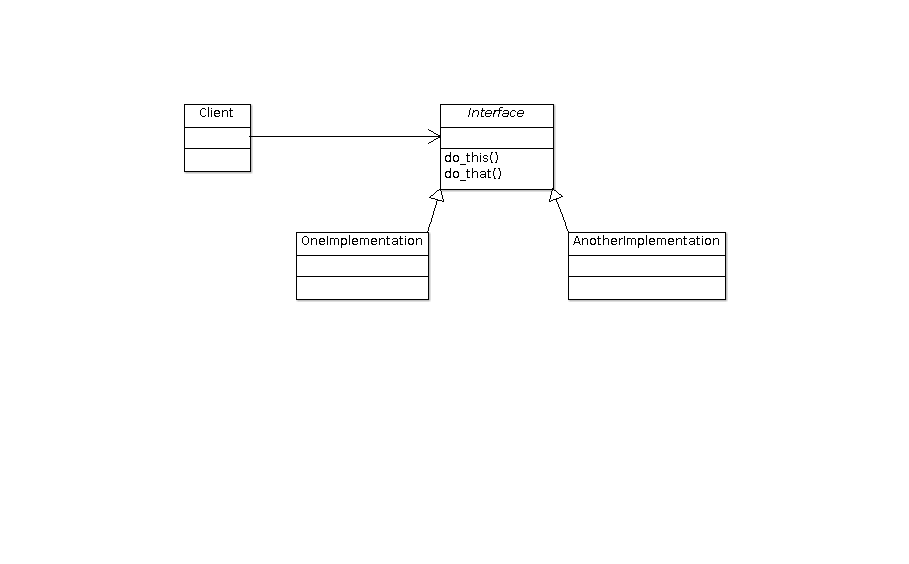
\includegraphics[height=0.9\textheight]{function-classic-polymorphism.png}
    \end{center}
  \end{block}

\end{frame}

% ---------------------------------------------------------------------------
\begin{frame}
  \frametitle{Classic Polymorphism: Upsides}

  \textbf{Polymorphism} is well understood:

  \begin{itemize}
  \item \textit{Late binding}: client does not know the exact type
    that is being used
  \item \textit{Interfaces} describe relationships in almost human
    language --- \textit{if done right}
  \item \textit{Software Architecture} --- \textit{if done right} ---
    is almost self-explanatory
  \item \textit{Design Patterns} are described (and mostly implemented
    as well) in such a way
  \item Also available in other languages
    \begin{itemize}
    \item For example Java explicitly distinguishes between
      \textit{interface} and \textit{implementation}
    \end{itemize}
  \end{itemize}
  
\end{frame}

% ---------------------------------------------------------------------------
\begin{frame}
  \frametitle{Classic Polymorphism: Technical Downsides}

  \textbf{There are purely technical downsides} (in C++ at least)

  \begin{itemize}
  \item Runtime overhead
    \begin{itemize}
    \item Not knowing the exact type implies \textit{indirect call}
      (function pointer/trampoline)
    \end{itemize}
  \item Code size
    \begin{itemize}
    \item If one writes \texttt{virtual}, a whole bunch of code is
      generated (Runtime Type Information --- RTTI)
    \item Type is not POD (\textit{plain old data}) anymore
    \end{itemize}
  \end{itemize}
  
\end{frame}

% ---------------------------------------------------------------------------
\begin{frame}
  \frametitle{Classic Polymorphism: More Downsides}

  \textbf{Metaphysical downsides} are harder to come by:
  \textbf{readability} again

  \begin{itemize}
  \item Provided that logging has no architectural relevance ...
  \item I have two functions which are similar in purpose, but
    otherwise unrelated. How can I arrange for client code to use
    these interchangeably?
    \begin{itemize}
    \item Why can't I \textit{just use} them?
    \item I don't want to instantiate client code from a template!
    \item Do I really want to craft an interface for client code to
      use?
    \end{itemize}
  \item I have a class that has similar purpose as the functions
    \begin{itemize}
    \item Client code wants to just call it
    \end{itemize}
  \item I want to \textit{adapt} all these!
  \item Sound like the solution is \texttt{std::bind}
  \item $\to$ Wrong: \texttt{std::bind} objects don't share a type
  \end{itemize}

  (Teacher's note: \texttt{classic-polymorphism-logger.cc})

\end{frame}

% ---------------------------------------------------------------------------
\begin{frame}[fragile]
  \frametitle{\texttt{std::function} to the Rescue (1)}

  \begin{itemize}
  \item \textbf{One type} to rule them all!
  \item $\to$ \textit{Any} callable with same signature
  \end{itemize}

  \begin{block}{Function object}
\begin{verbatim}
std::function<int(int, int)> foo_func;
\end{verbatim}
  \end{block}

  \begin{block}{Trivial: plain function}
\begin{verbatim}
int foo(int a, int b) { ... }
foo_func = foo;
\end{verbatim}
  \end{block}

\end{frame}

% ---------------------------------------------------------------------------
\begin{frame}[fragile]
  \frametitle{\texttt{std::function} to the Rescue (2)}

  \begin{block}{Any \texttt{std::bind} object}
\begin{verbatim}
struct bar {
    int foo(int a, int b) { ... }
};
foo_func = std::bind(&bar::foo, &bar,
       std::placeholders::_1, std::placeholders::_2);
\end{verbatim}
  \end{block}

  \begin{block}{Lambda}
\begin{verbatim}
foo_func = [](int a, int b) -> int { ... };
\end{verbatim}
  \end{block}
  
\end{frame}

% ---------------------------------------------------------------------------
\begin{frame}[fragile]
  \frametitle{\texttt{std::function}: Last Words}

  \textbf{Upsides}

  \begin{itemize}
  \item \textit{Lightweight Polymorphism}: no code explosion
  \item Unlike \textit{heavyweight polymorphism}, no dynamic
    allocation appropriate
    \begin{itemize}
    \item Although a \texttt{std::function} object can hold
      polymorphic callables, it is always the same size
    \end{itemize}
  \end{itemize}

  \textbf{Downsides}

  \begin{itemize}
  \item \textit{Runtime overhead} due to indirect call
    \begin{itemize}
    \item Processor support makes them just as fast as direct function
      calls
    \item \textit{But:} no inlining possible
    \end{itemize}
  \item \textit{Readability} again ...
    \begin{itemize}
    \item This is not OO!
    \item \textit{Architectural intentions} not at all obvious through
      quick inline adaptations
    \end{itemize}
  \end{itemize}
  
\end{frame}
